% TACL draft generated by paper/journal/build_journal.py.
% Needs tacl2021v1.sty from https://transacl.org/tacl-submission-templates/ in the same folder.
\documentclass[11pt,a4paper]{article}
\usepackage{times,latexsym}
\usepackage{url}
\usepackage[T1]{fontenc}
\usepackage[]{tacl2021v1}
\usepackage{xspace,mfirstuc,tabulary}
\usepackage{amsmath,amssymb,amsthm,graphicx,booktabs}
\newtheorem{theorem}{Theorem}
\newtheorem{proposition}[theorem]{Proposition}
\newtheorem{remark}{Remark}

\title{Auditing Language Model Answers Against Sources: Deterministic Verdict Rules, Provable Properties, and a Validation on FEVER}
\author{Piush Kole \\ Department of Computer Science, Christ University \\ {piushkole@msds.christuniversity.in} \\And Thrilok M \\ Department of Computer Science, Christ University \\ {thrilok.m@msds.christuniversity.in}}
\date{}
\begin{document}
\maketitle
\begin{abstract}
People read answers written by language models in their web browser, where a specific falsehood looks like a specific fact. We study an audit that splits an answer into claims, retrieves sources, records what each source says about each claim together with a verbatim quote, and maps these per-source stances to one of five verdicts by deterministic rules. We prove that the rules are exhaustive, order-invariant, symmetric and monotone, and that every assertion of truth or falsity rests on a verified quote. We also show, with proof, that a representation-density score used in earlier work reduces to a nearest-neighbour distance when claims are scored one at a time, and that an entropy-based uncertainty score is high whenever many sources match a claim about equally well, whether or not they agree. On 100 balanced FEVER claims, with full confusion matrices and paired exact tests, Wikipedia retrieval raised accuracy on SUPPORTS and REFUTES claims from 66.7\% to 79.7\% (paired p = 0.064), a pooled entailment score never abstained, and a first per-source variant abstained (61.3\% recall) at a significant cost in decisive accuracy (p < 0.001). A protocol for comparing several commercial models under one fixed checker is specified; it has not been run.
\end{abstract}

\section{Introduction}

Language models answer questions fluently and with specifics: names, dates, figures. A reader has no marker that separates a recalled fact from an invented one, and surveys of generation research document that models state unsupported or contradicted content with confidence \citep{ji2023}. Larger models can reproduce common human misconceptions more often, not less \citep{lin2022}. Checking what a model said against sources is therefore a practical need at the moment of reading, not only a benchmark task.

Automated fact-checking research supplies the components: claim detection, evidence retrieval, verdict prediction and justification \citep{guo2022}. Most published systems assume claims arrive already isolated and evidence comes from a fixed corpus \citep{thorne2018}. A deployed audit has neither. It must split a paragraph into claims, find evidence for each, and report a result that a reader can inspect. Two properties matter more in that setting than a point on a leaderboard. The first is auditability: for every verdict the reader should be able to see which sentence in which source decided it. The second is honesty about absence: a search that failed, a source that was not found, and a source that disagrees must not be collapsed into one outcome.

We make five contributions.

\begin{itemize}
\item A verdict procedure over per-source stances with a verbatim quote requirement, with five outcomes (Section 4).
\item Five properties of the procedure and of two scores from earlier work, each with a proof (Section 5) and each checked mechanically against the code (Section 5.6).
\item A validation on FEVER with complete confusion matrices, Wilson intervals and paired exact tests, including a failure analysis of a first per-source variant (Section 6).
\item An explicit failure semantics in which an outage is an error for the affected claim and never an empty result (Section 4.1).
\item A cross-model audit protocol with a fixed checker, a prompt list and a spending-bounded script, specified in full but not yet run (Section 7).
\end{itemize}

The work continues a study of whether representation-space density signals evidence insufficiency \citep{ss2026}. That study found the signal weak on FEVER (AUROC 0.5463), inverted on AVeriTeC (AUROC 0.2754) and at chance under a change of reference manifold. Sections 5.2 and 5.3 explain, for the two scores involved, why such a signal should not be expected to track support.

\section{Related Work}

\subsection{Automated fact-checking}

\citet{guo2022} survey the task as claim detection, evidence retrieval, verdict prediction and justification production. FEVER pairs Wikipedia-derived claims with the labels SUPPORTS, REFUTES and NOT ENOUGH INFO \citep{thorne2018}. AVeriTeC moves to real-world claims with evidence from the open web \citep{schlichtkrull2023}. We validate on FEVER because its labels allow abstention to be measured directly, and we discuss in the Limitations section what its Wikipedia origin does to the numbers.

\subsection{Factuality of generated text}

SelfCheckGPT detects hallucinated sentences by sampling a model several times and measuring consistency, without external evidence \citep{manakul2023}. FActScore decomposes a generation into atomic facts and reports the share a knowledge source supports \citep{min2023}. Our audit is close to FActScore in spirit; it differs in checking claims with a retrieval pipeline that can run in a reader's browser and in returning a verdict with a quote rather than a score.

\subsection{Distance, density and calibration}

Distance to a reference set is a common out-of-distribution score. We use cosine nearest-neighbour distance and Mahalanobis distance \citep{mahalanobis1936} with a shrunk covariance estimate \citep{ledoit2004} over sentence embeddings \citep{reimers2019,wang2020}. Split-conformal prediction turns a score into a calibrated decision without distributional assumptions \citep{angelopoulos2021}; our deployment carries that interface but does not fit it.

\subsection{Language models as judges}

Using one model to judge another is common and has known biases, including a preference for answers from the same family \citep{zheng2023}. We hold the checker fixed across audited models, which removes differences caused by the checker but not a bias of the checker.

\section{Problem Setting}

Let $x$ be a passage. A claim extractor returns claims $c_1,\dots,c_m$. For a claim $c$ a retriever returns sources $e_1,\dots,e_n$ with $n \ge 0$. A stance model returns, for each source, a stance $\sigma_i \in \{\text{supports},\text{refutes},\text{neutral},\text{irrelevant}\}$, a confidence $\kappa_i \in [0,1]$ and a quote $q_i$ that must occur in $e_i$. The audit output for $c$ is a verdict $v \in \mathcal{V} = \{\text{supported},\text{refuted},\text{mixed},\text{insufficient},\text{no\_sources}\}$.

To compare verdicts with FEVER labels we use the incidence matrix $\Phi \in \{0,1\}^{5 \times 4}$ whose rows are the five verdicts and whose columns are SUPPORTS, REFUTES, NOT ENOUGH INFO (NEI) and an extra column MIXED, so that a predicted label is the column in which a verdict's row has its one entry:

\begin{table}[t]
\centering
\[\begin{array}{lcccc}
 & \mathit{SUPPORTS} & \mathit{REFUTES} & \mathit{NEI} & \mathit{MIXED} \\
\mathit{supported} & \left[\begin{matrix} 1 & 0 & 0 & 0 \end{matrix}\right] \\
\mathit{refuted} & \left[\begin{matrix} 0 & 1 & 0 & 0 \end{matrix}\right] \\
\mathit{mixed} & \left[\begin{matrix} 0 & 0 & 0 & 1 \end{matrix}\right] \\
\mathit{insufficient} & \left[\begin{matrix} 0 & 0 & 1 & 0 \end{matrix}\right] \\
\mathit{no\_sources} & \left[\begin{matrix} 0 & 0 & 1 & 0 \end{matrix}\right] \\
\end{array}\]
\caption{Mapping $\Phi$ from verdicts to labels.}
\par{\scriptsize Mixed is a label of its own and always counts as wrong against a three-class gold label.}
\end{table}

\section{System and Verdict Rules}

\subsection{Claim extraction, retrieval and failure semantics}

A language model returns the checkable assertions in $x$ as self-contained statements. Names, numbers and dates are kept as written; opinions, questions and predictions are skipped; duplicates are removed and identifiers are reassigned by the service. A normalised form with a core entity and predicate is used only to build search queries, because normalisation can drop the detail that makes a claim false. Two retrievers run concurrently: a Wikipedia retriever (two MediaWiki searches, lead-section extracts) and OpenAlex \citep{priem2022}. Results are merged and deduplicated by identifier and text.

Failure is explicit. If one retriever fails while another returns sources, the claim proceeds. If every retriever failed, or one failed and none returned anything, the claim fails with an error. A connection that closes before the terminal stream event marks unfinished claims as failed. A failed claim is therefore never displayed as the absence of evidence (Figure 1).

\begin{figure}[t]
\centering
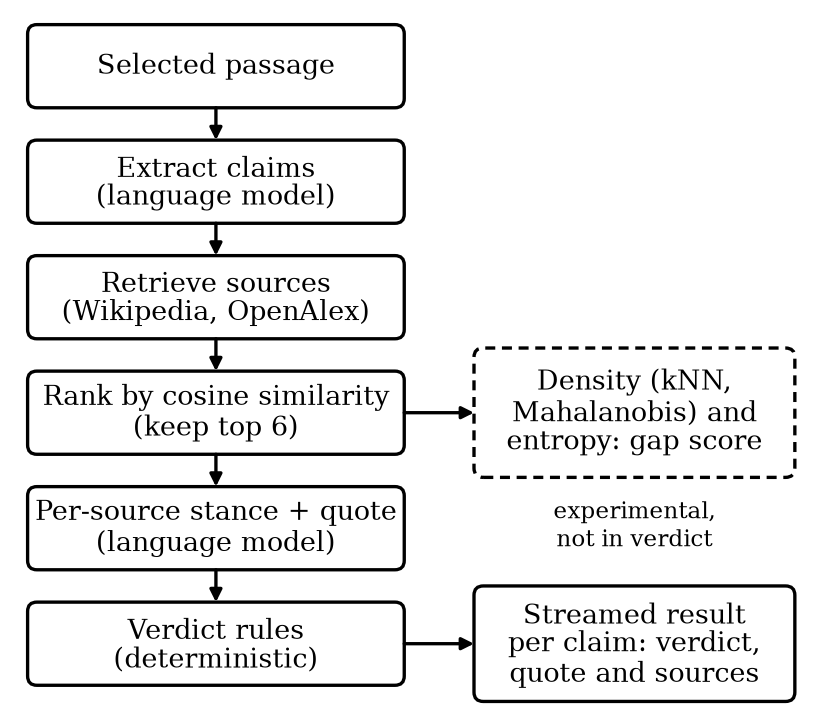
\includegraphics[width=\columnwidth]{figs/pipeline.png}
\caption{System overview. Solid boxes decide the verdict. The dashed box is computed alongside it and shown only in research mode.}
\end{figure}

\subsection{Ranking}

With sentence embeddings $\mathbf{u}_c$ and $\mathbf{u}_{e_i}$ of the claim and a source, sources are ordered by cosine similarity

\begin{equation}
s_i = \frac{\mathbf{u}_c \cdot \mathbf{u}_{e_i}}{\lVert \mathbf{u}_c \rVert\, \lVert \mathbf{u}_{e_i} \rVert}
\end{equation}

and the top $K=6$ are kept. A source with $s_i < 0.15$ is dropped only if it ranks below the first two, so a poor embedding match alone can never empty a non-empty list.

\subsection{Stance assessment}

One model call returns $(\sigma_i,\kappa_i,q_i)$ for every kept source. Support requires every specific detail of the claim (names, dates, places, numbers, categories) to be confirmed; a different year or category is a conflict. A stance of supports or refutes is kept only if $q_i$ occurs verbatim in the source after whitespace and case normalisation; otherwise it is downgraded to neutral. With thresholds $\theta = 0.5$ and $\gamma = 0.8$ define the counted sets and the qualifying predicate

\begin{equation}
\begin{aligned}
\mathcal{P} = \{\, i : \sigma_i = \text{supports},\ \kappa_i \ge \theta,\ q_i \ne \emptyset \,\}, \\
\mathcal{N} = \{\, i : \sigma_i = \text{refutes},\ \kappa_i \ge \theta,\ q_i \ne \emptyset \,\}
\end{aligned}
\end{equation}

\begin{equation}
Q(T) = \bigl(|T| \ge 2\bigr) \lor \bigl(|T| = 1 \land \max_{i \in T} \kappa_i \ge \gamma\bigr)
\end{equation}

\subsection{Verdict rules}

The verdict is the first rule that applies:

\begin{itemize}
\item R1: no sources if $n = 0$.
\item R2: mixed if $\mathcal{P} \ne \emptyset$, $\mathcal{N} \ne \emptyset$ and $Q(\mathcal{P}) \lor Q(\mathcal{N})$.
\item R3: supported if $Q(\mathcal{P})$.
\item R4: refuted if $Q(\mathcal{N})$.
\item R5: insufficient otherwise, marked as leaning towards a side that has counted sources when the other side has none.
\end{itemize}

Let $\mathcal{R}$ be the sources whose stance is not irrelevant. For display, confidence-weighted shares are

\begin{equation}
\begin{aligned}
\mathrm{supp} = \frac{\sum_{i \in \mathcal{R},\, \sigma_i = \text{supports}} \kappa_i}{\sum_{i \in \mathcal{R}} \kappa_i}, \\
\mathrm{conf} = \frac{\sum_{i \in \mathcal{R},\, \sigma_i = \text{refutes}} \kappa_i}{\sum_{i \in \mathcal{R}} \kappa_i}
\end{aligned}
\end{equation}

\begin{figure}[t]
\centering
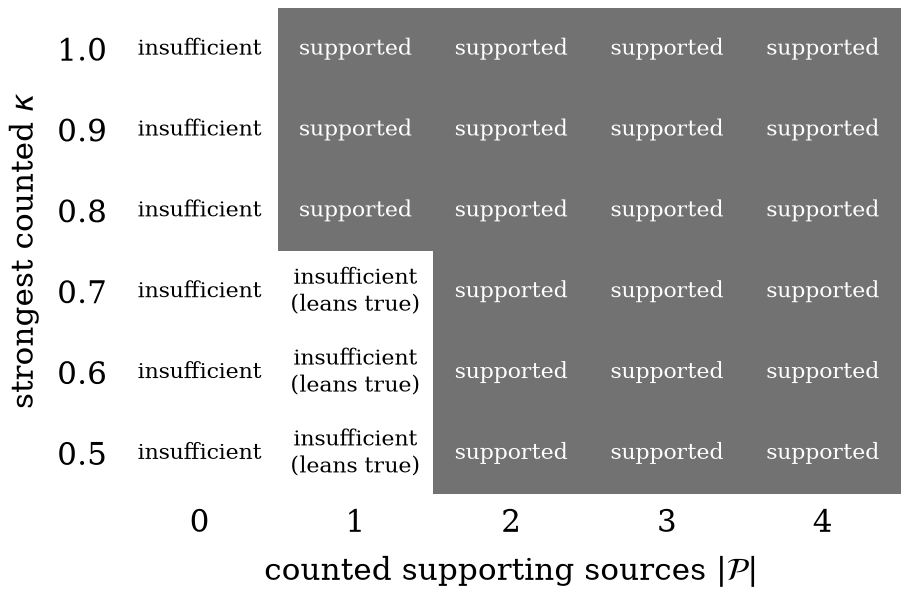
\includegraphics[width=\columnwidth]{journal_figs/regions.png}
\caption{Verdict as a function of the number of counted supporting sources and the strongest counted confidence, with no counted refutation. One source qualifies only at confidence 0.8 or higher.}
\end{figure}

\subsection{Experimental representation-space signals}

Two signals from the earlier study are computed for every claim and shown only in research mode. With claim embedding $\mathbf{q}$ and its $k=5$ nearest neighbours $\mathbf{r}_{(1)},\dots,\mathbf{r}_{(k)}$ in a reference set of 10,000 FEVER claim embeddings, the neighbourhood distance is

\begin{equation}
d_k(\mathbf{q}) = \frac{1}{k}\sum_{j=1}^{k}\bigl(1-\cos(\mathbf{q},\mathbf{r}_{(j)})\bigr)
\end{equation}

The Mahalanobis distance uses a shrunk covariance of the reference set:

\begin{equation}
\begin{aligned}
d_M(\mathbf{q}) = \sqrt{(\mathbf{q}-\boldsymbol{\mu})^{\top}\hat{\Sigma}^{-1}(\mathbf{q}-\boldsymbol{\mu})}, \\
\hat{\Sigma} = (1-\delta)\,S + \delta\,\bar{\mu}\,I,\quad \bar{\mu} = \frac{\operatorname{tr}(S)}{p}
\end{aligned}
\end{equation}

The density score normalises $d_M$ by its maximum over the batch $B$ of queries scored together:

\begin{equation}
\rho(\mathbf{q}) = \frac{1}{2}\left(d_k(\mathbf{q}) + \frac{d_M(\mathbf{q})}{\max_{\mathbf{q}' \in B} d_M(\mathbf{q}') + \varepsilon}\right)
\end{equation}

The second signal is the normalised entropy of a softmax over the similarities $s_1,\dots,s_N$ with temperature $\tau = 0.1$:

\begin{equation}
\begin{aligned}
p_i = \frac{\exp(s_i/\tau)}{\sum_{j=1}^{N}\exp(s_j/\tau)}, \\
U = -\frac{1}{\ln N}\sum_{i=1}^{N} p_i \ln p_i
\end{aligned}
\end{equation}

with $U=1$ for $N=0$ and $U=0$ for $N=1$. The experimental gap score is $G = (\rho + U)/2$.

\section{Properties and Proofs}

This section states five properties. Each proof is short and uses only the definitions above. Section 5.6 describes how each statement is also checked against the implementation.

\subsection{The verdict rules}

\begin{theorem}[Verdict rules]
Let $S$ be a finite list of assessed sources and let $\mathcal{P}$, $\mathcal{N}$ be its counted sets. Then: (a) $v(S)$ is the unique verdict with $v=\text{no\_sources}$ iff $S=\emptyset$; $\text{mixed}$ iff $\mathcal{P}\ne\emptyset$, $\mathcal{N}\ne\emptyset$ and $Q(\mathcal{P})\lor Q(\mathcal{N})$; $\text{supported}$ iff $Q(\mathcal{P})$ and $\mathcal{N}=\emptyset$; $\text{refuted}$ iff $Q(\mathcal{N})$ and $\mathcal{P}=\emptyset$; $\text{insufficient}$ iff $S\ne\emptyset$, $\neg Q(\mathcal{P})$ and $\neg Q(\mathcal{N})$. For non-empty $S$: (b) $v$ is invariant under permutations of $S$ and under appending sources that are not counted; (c) exchanging the roles of supports and refutes exchanges supported and refuted and fixes the other three verdicts; (d) if $v(S)=\text{supported}$ and a source $s$ is appended, then $v=\text{mixed}$ if $s$ is a counted refutation and $v=\text{supported}$ otherwise; (e) if $v(S) \in \{\text{supported},\text{refuted},\text{mixed}\}$ then some source has $\kappa_i \ge \theta$ and a quote that occurs verbatim in its text.
\end{theorem}

\begin{proof}
(a) The rules are tried in order. R1 fires exactly when $n=0$. Suppose $n \ge 1$. R2 fires exactly when its stated condition holds. Assume R2 does not fire. R3 fires iff $Q(\mathcal{P})$. Then $\mathcal{P}\ne\emptyset$ (since $Q(\emptyset)$ is false), so $\mathcal{N}=\emptyset$, because otherwise R2 would have fired; conversely $\mathcal{N}=\emptyset$ makes R2 false. Hence R3 yields supported iff $Q(\mathcal{P}) \land \mathcal{N}=\emptyset$. The argument for R4 is symmetric: $Q(\mathcal{N})$ forces $\mathcal{N}\ne\emptyset$, non-firing of R2 forces $\mathcal{P}=\emptyset$, and then R3 cannot fire. R5 applies when none of R2 to R4 do. If $Q(\mathcal{P})$ holds then R2 or R3 fires, and if $Q(\mathcal{N})$ holds then R2 or R4 fires; conversely if both are false, R2 to R4 all fail. So R5 applies iff $\neg Q(\mathcal{P}) \land \neg Q(\mathcal{N})$. The conditions are mutually exclusive by construction, so exactly one verdict results.

(b) The rules read $S$ only through $n \ge 1$ and the multisets of confidences in $\mathcal{P}$ and $\mathcal{N}$. Permuting $S$ leaves these unchanged. A source that is not counted belongs to neither set, and $n \ge 1$ continues to hold.

(c) Exchanging supports and refutes exchanges $\mathcal{P}$ and $\mathcal{N}$. The conditions for mixed and insufficient are symmetric in $(\mathcal{P},\mathcal{N})$, and those for supported and refuted are exchanged.

(d) By (a), $v(S)=\text{supported}$ gives $Q(\mathcal{P})$ and $\mathcal{N}=\emptyset$. If $s$ is a counted refutation, the new $\mathcal{N}$ is non-empty and $\mathcal{P}$ is unchanged, so $v$ is mixed by (a). Otherwise $\mathcal{N}$ stays empty and $\mathcal{P}$ can only grow. $Q$ is monotone under adding members: if $|\mathcal{P}| \ge 2$ it stays so, and if $|\mathcal{P}|=1$ with $\kappa \ge \gamma$ then either a member is added, giving size two, or the set is unchanged. Hence $Q(\mathcal{P})$ still holds and $v$ stays supported.

(e) By (a), these verdicts require $Q(\mathcal{P})$ or $Q(\mathcal{N})$, and $Q(T)$ is false for $T = \emptyset$. A member of a counted set has $\kappa_i \ge \theta$ and a non-empty quote, which the stance step verified to occur in the source.
\end{proof}

\begin{remark}
Part (e) is the audit property: the system cannot assert that a claim is true, false or disputed without a quote that a reader can find in the source. A corollary is that if every confidence is below $\theta$ the verdict is no sources or insufficient.
\end{remark}

\subsection{Entropy of the similarity distribution}

\begin{proposition}[Behaviour of $U$]
Let $N \ge 2$, similarities $s_1,\dots,s_N$ and $\tau > 0$, with $U$ as in the definition above. (a) $0 \le U \le 1$, and $U = 1$ iff all $s_i$ are equal. (b) $U$ is non-decreasing in $\tau$. (c) If $\delta = \max_i s_i - \min_i s_i$ then $U \ge 1 - \delta/(\tau \ln N)$.
\end{proposition}

\begin{proof}
(a) $H = -\sum p_i \ln p_i \le \ln N$ with equality iff $p$ is uniform, by Gibbs' inequality \citep{cover2006}. Since $p_i \propto e^{s_i/\tau}$, $p$ is uniform iff all $s_i$ are equal. $H \ge 0$ gives $U \ge 0$.

(b) Write $\beta = 1/\tau$, $Z(\beta) = \sum_i e^{\beta s_i}$ and $\mathbb{E}$ for expectation under $p$. Then $H = \ln Z - \beta\,\mathbb{E}[s]$. Using $\mathrm{d}\ln Z/\mathrm{d}\beta = \mathbb{E}[s]$ and $\mathrm{d}\,\mathbb{E}[s]/\mathrm{d}\beta = \operatorname{Var}_p(s)$ we get $\mathrm{d}H/\mathrm{d}\beta = -\beta \operatorname{Var}_p(s) \le 0$. So $H$ is non-increasing in $\beta$, hence non-decreasing in $\tau$.

(c) Let $u$ be the uniform distribution. $\ln N - H = D(p \Vert u) = \sum p_i \ln(N p_i) \le \ln(N \max_i p_i)$. Since $s_i - s_{\min} \le \delta$, $p_i = e^{s_i/\tau}/\sum_j e^{s_j/\tau} \le e^{\delta/\tau}/N$. Hence $\ln N - H \le \delta/\tau$, and dividing by $\ln N$ gives the bound.
\end{proof}

\begin{remark}
Figure 3 shows the bound. For $N = 10$ and $\tau = 0.1$, sources whose similarities lie within $0.05$ of each other give $U \ge 0.78$. $U$ measures how evenly sources match the claim. It cannot distinguish sources that agree with a claim from sources that merely resemble it.
\end{remark}

\begin{figure}[t]
\centering
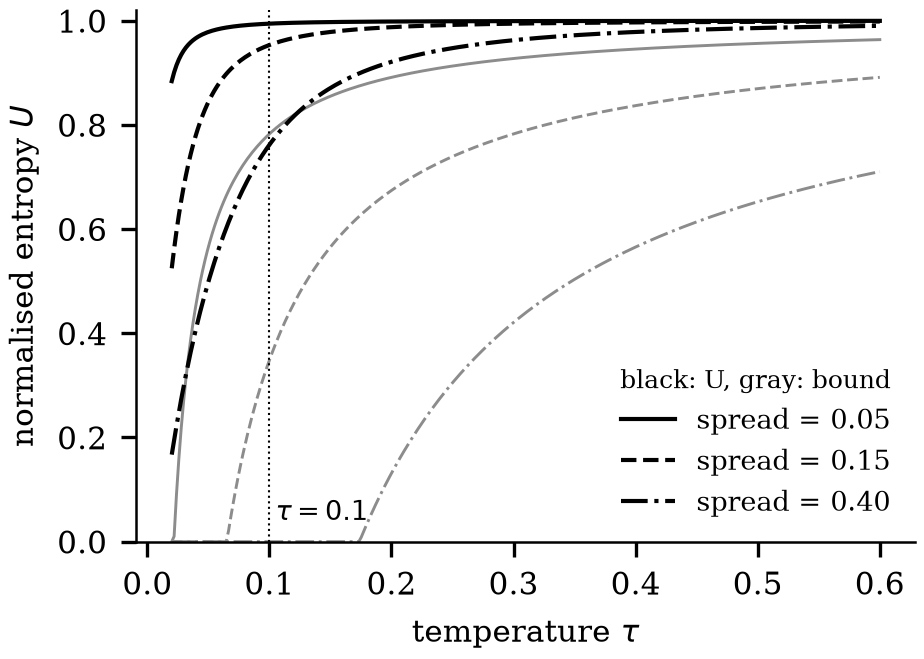
\includegraphics[width=\columnwidth]{journal_figs/entropy.png}
\caption{Normalised entropy $U$ against temperature for $N = 10$ similarities spread over 0.05, 0.15 and 0.40 (black) with the lower bound of Proposition 2(c) (gray). The dotted line marks the deployed temperature.}
\end{figure}

\subsection{The density score for a single query}

\begin{proposition}[Degeneracy of batch normalisation]
Let the batch be a single query, $B = \{\mathbf{q}\}$, with $d_M(\mathbf{q}) > 0$ and $\varepsilon > 0$. Then $\rho(\mathbf{q}) = (d_k + 1)/2 - \varepsilon / (2(d_M + \varepsilon))$, so $0 \le (d_k+1)/2 - \rho < \varepsilon/(2 d_M)$. The retrieval confidence $\max(0, 1-\rho)$ is at most $1/2 + \varepsilon/(2 d_M)$. If two queries satisfy $d_k(\mathbf{q}_2) - d_k(\mathbf{q}_1) > \varepsilon$ then $\rho(\mathbf{q}_1) < \rho(\mathbf{q}_2)$.
\end{proposition}

\begin{proof}
For $B = \{\mathbf{q}\}$ the maximum in the denominator is $d_M + \varepsilon$ itself, so the second term is $d_M/(d_M+\varepsilon) = 1 - \varepsilon/(d_M+\varepsilon)$. Substituting gives the expression for $\rho$ and the first inequality, since $0 < \varepsilon/(d_M+\varepsilon) < \varepsilon/d_M$. As $d_k \ge 0$, $1 - \rho = (1-d_k)/2 + \varepsilon/(2(d_M+\varepsilon)) \le 1/2 + \varepsilon/(2 d_M)$. For the last claim, $2\rho(\mathbf{q}_i) = d_k(\mathbf{q}_i) + 1 - e_i$ with $e_i \in [0, \varepsilon)$, so $2\rho(\mathbf{q}_2) - 2\rho(\mathbf{q}_1) > \varepsilon - (e_2 - e_1) > 0$.
\end{proof}

\begin{remark}
Scored one claim at a time, as in the earlier experiments and here, $\rho$ orders claims exactly as $d_k$ does, apart from differences below $\varepsilon = 10^{-9}$, so the Mahalanobis term cannot change any ranking metric such as AUROC. Retrieval confidence is capped near $1/2$ by construction.
\end{remark}

\subsection{Conditioning of the shrunk covariance}

\begin{proposition}[Shrinkage]
Let $S \in \mathbb{R}^{p \times p}$ be symmetric positive semidefinite with $\bar{\mu} = \operatorname{tr}(S)/p > 0$ and let $\delta \in (0, 1]$. Then $\hat{\Sigma} = (1-\delta)S + \delta\bar{\mu}I$ is positive definite with all eigenvalues at least $\delta\bar{\mu}$, its spectral condition number satisfies $\kappa_2(\hat{\Sigma}) \le 1 + (1-\delta)p/\delta$, and $d_M(\mathbf{q}) \le \lVert \mathbf{q} - \boldsymbol{\mu} \rVert / \sqrt{\delta\bar{\mu}}$.
\end{proposition}

\begin{proof}
$S$ has an orthonormal eigenbasis with eigenvalues $\lambda_j \ge 0$ \citep{horn2013}. $\hat{\Sigma}$ has the same eigenvectors, with eigenvalues $(1-\delta)\lambda_j + \delta\bar{\mu}$, which lie in $[\delta\bar{\mu},\ (1-\delta)\lambda_{\max} + \delta\bar{\mu}]$. Therefore $\hat{\Sigma}$ is positive definite and $\kappa_2 \le 1 + (1-\delta)\lambda_{\max}/(\delta\bar{\mu})$. All $\lambda_j \ge 0$ gives $\lambda_{\max} \le \operatorname{tr}(S) = p\bar{\mu}$, hence $\kappa_2 \le 1 + (1-\delta)p/\delta$. Finally $d_M^2 = \mathbf{v}^{\top}\hat{\Sigma}^{-1}\mathbf{v} \le \lVert\mathbf{v}\rVert^2/\lambda_{\min}(\hat{\Sigma}) \le \lVert\mathbf{v}\rVert^2/(\delta\bar{\mu})$.
\end{proof}

\begin{remark}
The bound holds even when fewer reference points than dimensions make $S$ singular, which is the case the shrinkage estimator is designed for \citep{ledoit2004}. Appendix A.3 works a $2 \times 2$ example.
\end{remark}

\subsection{Wilson intervals}

\begin{proposition}[Wilson interval]
For $k$ successes in $n$ trials with $\hat{p} = k/n$ and $z > 0$, the set of $p$ with $(\hat{p}-p)^2 \le z^2 p(1-p)/n$ is an interval $[p_-, p_+] \subseteq [0,1]$ that contains $\hat{p}$; its endpoints are the Wilson limits.
\end{proposition}

\begin{proof}
Let $f(p) = (\hat{p}-p)^2 - z^2p(1-p)/n$. It is a convex quadratic with leading coefficient $1 + z^2/n > 0$. Moreover $f(0) = \hat{p}^2 \ge 0$, $f(1) = (1-\hat{p})^2 \ge 0$ and $f(\hat{p}) = -z^2\hat{p}(1-\hat{p})/n \le 0$. A convex function that is non-positive at $\hat{p} \in [0,1]$ and non-negative at $0$ and $1$ has one root in $[0,\hat{p}]$ and one in $[\hat{p},1]$, and is non-positive between them. Solving $f(p)=0$ gives the Wilson limits \citep{wilson1927}.
\end{proof}

\subsection{Mechanical verification}

Each statement above is also tested against the code it describes. Theorem 1 is checked on every configuration of up to three sources over 30 stance, confidence and quote combinations (27,930 configurations), plus 15,000 random configurations of four to seven sources, using the deployed aggregation function; Proposition 2 and 4 are checked on random inputs against the deployed entropy module and scikit-learn's Ledoit--Wolf estimator; Proposition 3 against the deployed density estimator. These checks are not proofs, but they fail if a statement and the implementation drift apart, and they found no counterexample.

\section{Validation on FEVER}

\subsection{Setup}

We sample claims from the FEVER paper development split, balanced over SUPPORTS, REFUTES and NEI (seed 42), deduplicated by claim identifier. Three variants are run on the same claims: a pooled variant that sends all sources in one call and obtains an entailment score $e$ and a contradiction score $c$ (refuted if $c \ge 0.5$, supported if $e \ge 0.6$, insufficient otherwise), with OpenAlex or Wikipedia retrieval; and the per-source variant of Section 4 with Wikipedia retrieval and its first prompt. The OpenAlex run covered 150 sampled claims, but 50 failed when the anonymous request budget was exhausted; every variant is reported on the 100 claims that run scored. Of these, 33 are SUPPORTS, 36 REFUTES and 31 NEI, so 69 are decisive.

With confusion matrix $M \in \mathbb{N}^{3 \times 4}$ (rows gold, columns predicted), accuracy, precision and recall are

\begin{equation}
\begin{aligned}
\mathrm{Acc} = \frac{\sum_{c=1}^{3} M_{cc}}{\sum_{c,j} M_{cj}}, \\
P_c = \frac{M_{cc}}{\sum_{g=1}^{3} M_{gc}}, \\
R_c = \frac{M_{cc}}{\sum_{j=1}^{4} M_{cj}}
\end{aligned}
\end{equation}

with $F1_c = 2P_cR_c/(P_c+R_c)$ and macro-$F1$ the mean over the three gold classes. Decisive accuracy is $(M_{11}+M_{22})/(\sum_j M_{1j} + \sum_j M_{2j})$. Proportions carry 95\% Wilson intervals (Proposition 5). Variants are compared on the same claims with an exact two-sided McNemar test on the discordant pairs and a paired bootstrap of 4,000 resamples for the difference.

\subsection{Results}

Figure 4 and the matrices below give the full outcome of each variant.

\begin{table}[t]
\centering
\[\begin{array}{lcccc}
 & \mathit{S} & \mathit{R} & \mathit{N} & \mathit{M} \\
\mathit{SUPPORTS} & \left[\begin{matrix} 15 & 9 & 9 & 0 \end{matrix}\right] \\
\mathit{REFUTES} & \left[\begin{matrix} 3 & 31 & 2 & 0 \end{matrix}\right] \\
\mathit{NEI} & \left[\begin{matrix} 2 & 24 & 5 & 0 \end{matrix}\right] \\
\end{array}\]
\caption{Confusion matrix $M$, pooled score with OpenAlex (baseline).}
\end{table}

\begin{table}[t]
\centering
\[\begin{array}{lcccc}
 & \mathit{S} & \mathit{R} & \mathit{N} & \mathit{M} \\
\mathit{SUPPORTS} & \left[\begin{matrix} 24 & 8 & 1 & 0 \end{matrix}\right] \\
\mathit{REFUTES} & \left[\begin{matrix} 4 & 31 & 1 & 0 \end{matrix}\right] \\
\mathit{NEI} & \left[\begin{matrix} 6 & 25 & 0 & 0 \end{matrix}\right] \\
\end{array}\]
\caption{Confusion matrix $M$, pooled score with Wikipedia.}
\end{table}

\begin{table}[t]
\centering
\[\begin{array}{lcccc}
 & \mathit{S} & \mathit{R} & \mathit{N} & \mathit{M} \\
\mathit{SUPPORTS} & \left[\begin{matrix} 22 & 2 & 8 & 1 \end{matrix}\right] \\
\mathit{REFUTES} & \left[\begin{matrix} 13 & 12 & 10 & 1 \end{matrix}\right] \\
\mathit{NEI} & \left[\begin{matrix} 9 & 3 & 19 & 0 \end{matrix}\right] \\
\end{array}\]
\caption{Confusion matrix $M$, per-source stance with Wikipedia (first prompt).}
\par{\scriptsize Rows sum to 33, 36 and 31 in every matrix.}
\end{table}

\begin{figure}[t]
\centering
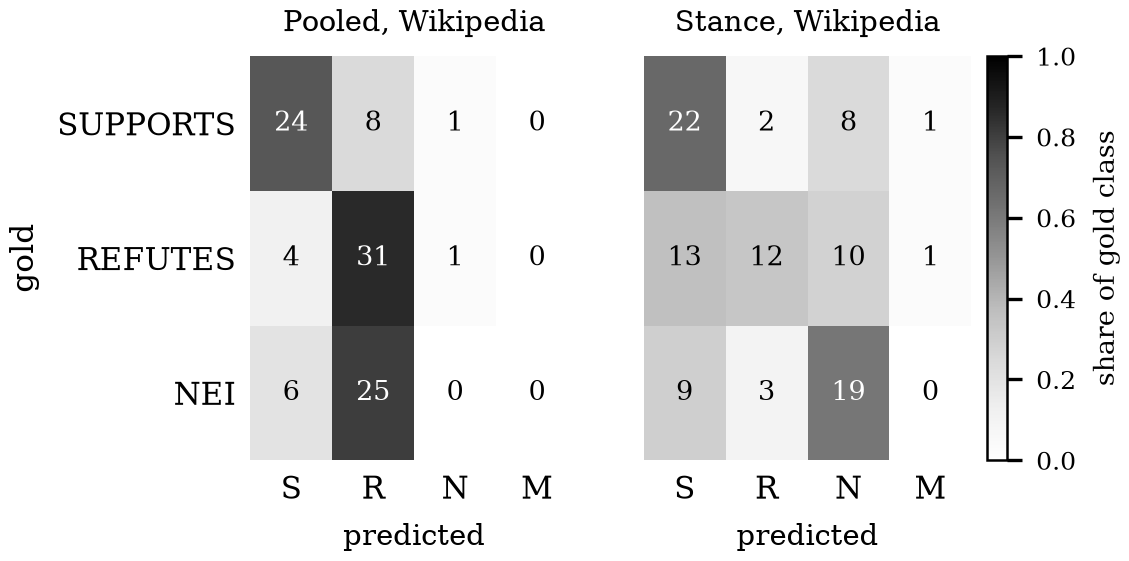
\includegraphics[width=\columnwidth]{journal_figs/confusion.png}
\caption{Row-normalised confusion matrices with counts for the two Wikipedia variants. S, R, N and M are SUPPORTS, REFUTES, NEI and MIXED.}
\end{figure}

\begin{table}[t]
\centering\footnotesize
\begin{tabular}{lcccc}
\toprule
Variant & Accuracy (95\% CI) & Macro F1 & Decisive acc. (95\% CI) & NEI recall \\
\midrule
Pooled, OpenAlex & 51.0 (41.3--60.6) & 0.466 & 66.7 (54.9--76.6) & 16.1 \\
Pooled, Wikipedia & 55.0 (45.2--64.4) & 0.445 & 79.7 (68.8--87.5) & 0.0 \\
Stance, Wikipedia & 53.0 (43.3--62.5) & 0.528 & 49.3 (37.8--60.8) & 61.3 \\
\bottomrule
\end{tabular}
\caption{Verdict validation on 100 FEVER claims, computed from the matrices above.}
\par{\scriptsize Percent, except macro F1. Decisive accuracy is over the 69 SUPPORTS and REFUTES claims.}
\end{table}

\begin{figure}[t]
\centering
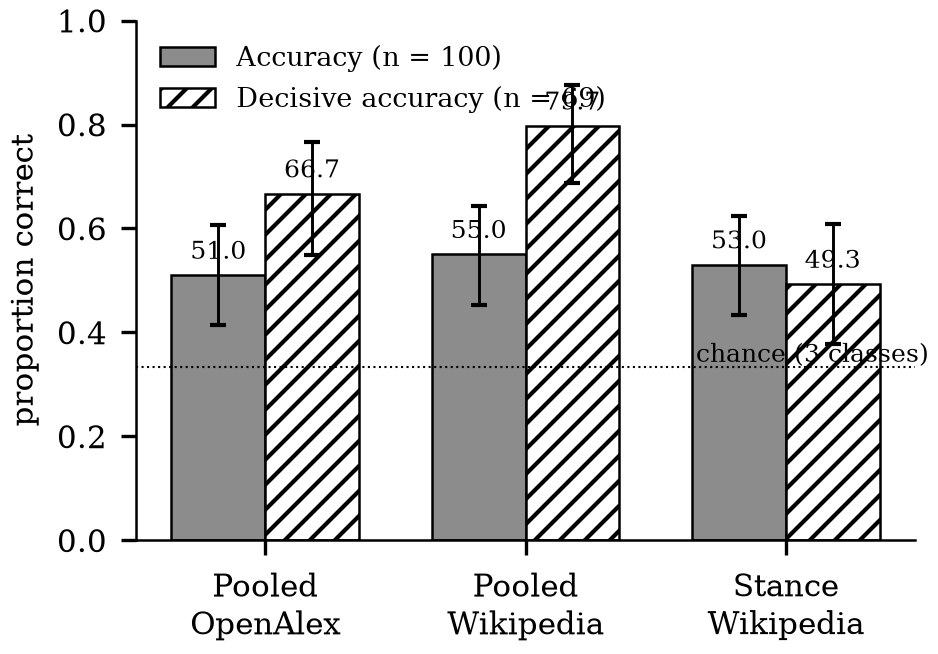
\includegraphics[width=\columnwidth]{journal_figs/accuracy.png}
\caption{Overall and decisive accuracy with 95\% Wilson intervals. The dotted line is the three-class chance level.}
\end{figure}

\begin{table}[t]
\centering\footnotesize
\begin{tabular}{lcccc}
\toprule
A vs B & Claims (n) & A only / B only & Diff. (95\% CI), points & p \\
\midrule
PW vs PO & all (100) & 14 / 10 & +4.0 (-6.0 to +14.0) & 0.541 \\
PW vs PO & decisive (69) & 14 / 5 & +13.0 (+1.4 to +24.6) & 0.064 \\
SW vs PW & all (100) & 24 / 26 & -2.0 (-16.0 to +12.0) & 0.888 \\
SW vs PW & decisive (69) & 5 / 26 & -30.4 (-44.9 to -15.9) & 0.0002 \\
SW vs PO & all (100) & 27 / 25 & +2.0 (-12.0 to +16.0) & 0.890 \\
SW vs PO & decisive (69) & 11 / 23 & -17.4 (-33.3 to 0.0) & 0.058 \\
\bottomrule
\end{tabular}
\caption{Paired comparisons on the same claims (exact McNemar test; paired bootstrap).}
\par{\scriptsize PO: pooled score with OpenAlex. PW: pooled score with Wikipedia. SW: per-source stance with Wikipedia. A only: claims A got right and B wrong; B only: the reverse. Six tests; with Bonferroni correction the threshold is 0.0083, which only the fourth row meets.}
\end{table}

\subsection{Analysis}

Three findings follow. First, Wikipedia retrieval raised decisive accuracy over scholarly-only retrieval by 13.0 points, but the paired test does not reach the 0.05 level ($p = 0.064$), and claims drawn from Wikipedia are expected to favour a Wikipedia retriever; we call the gain suggestive. Second, the pooled score never abstains: its NEI recall is 0\% with Wikipedia and it labelled 25 of 31 NEI claims as refuted. One entailment and one contradiction score cannot separate sources that do not mention a claim from sources that contradict it. Third, the first per-source variant abstains (NEI recall 61.3\%) but is significantly worse on decisive claims than the pooled score ($p = 0.0002$), while its overall accuracy is indistinguishable (24 against 26 discordant claims).

We inspected the 13 REFUTES claims that the per-source variant labelled supported. Two causes were ours. The stance call judged the model-normalised claim, which had dropped the detail that made the claim false (``The Monster is a restaurant by Eminem'' became ``The Monster is a restaurant''), and the prompt accepted near misses as support (1945 for 1946; a television series for a radio station). Both were corrected and a regression test fixes the first. A re-evaluation of the corrected prompt on a fresh sample was interrupted by an exhausted language-model account after 27 scored claims, so no conclusion is drawn about the corrected variant.

\section{Cross-Model Audit Protocol}

A fixed list of 40 prompts covers five domains (32 prompts) and eight common-misconception questions. Each model answers every prompt at temperature zero with one system prompt, in three to five sentences. The planned models are GPT-4o, Claude Sonnet 4.5, Gemini 2.5 Pro and Flash, Llama 3.3 70B, DeepSeek Chat and Mistral Large, reached through one API gateway; versions are recorded in run metadata, and API models can differ from the consumer products that share their names. Each answer is split into claims and each claim is checked by the same pipeline, checker model and retrievers. For model $m$ with claim set $\mathcal{C}_m$ and verdict $v(c)$ the claim-level rate of a verdict $x$ and the share of answers containing a refuted claim are

\begin{equation}
R_m^{(x)} = \frac{\bigl|\{\, c \in \mathcal{C}_m : v(c) = x \,\}\bigr|}{|\mathcal{C}_m|}
\end{equation}

\begin{equation}
A_m = \frac{1}{|\mathcal{Q}|}\sum_{r \in \mathcal{Q}} \mathbb{1}\bigl[\exists\, c \in \mathcal{C}_{m,r} : v(c) = \text{refuted}\bigr]
\end{equation}

where $\mathcal{Q}$ is the prompt set. Claims within one answer are not independent, so a difference $\Delta = R_a^{(x)} - R_b^{(x)}$ is given with a paired bootstrap that resamples prompts \citep{efron1979}. Failed calls and failed checks are counted and reported, never scored. The script, prompt list and an upper cost estimate (about 1.6 US dollars) are part of the artefact. At the time of writing the language-model account had no credit, so the audit has not been run and no figures are reported or extrapolated.

\section{Conclusion}

An audit of language-model answers is useful when each verdict can be traced to a sentence and when absence is kept apart from failure. The rules we describe have these properties provably, and two scores from earlier work do not behave as their names suggest: a single-query density score is a nearest-neighbour distance, and an entropy score rewards redundancy. On FEVER, retrieval source mattered more than the aggregation rule for decisive claims, and a pooled score could not abstain. The next steps are to evaluate the corrected per-source prompt on a larger sample, to run the cross-model audit, and to compare verdicts with human judgements on audited answers.

\section*{Limitations}

A refuted claim is one that retrieved sources push against; it is evidence about the source pool and the checker, not a ground-truth label. The checker is a language model and may favour answers from its own family. FEVER claims were written from Wikipedia, which a Wikipedia retriever and the models may know, so only relative comparisons between variants are meaningful. NEI is a statement about the annotators' corpus, not about the open web. With 100 claims, intervals are about $\pm 10$ points. The corrected per-source prompt is not yet evaluated. Anonymous OpenAlex budgets are small; the system reports exhaustion as an error. Highlighting claims on a page works only for claims that appear word for word. Finally, the properties in Section 5 concern the rules, not the stance model: a confident, quoted, wrong stance yields a wrong verdict, and the quote requirement makes that error visible rather than impossible.

\section*{Acknowledgments}
The authors thank the maintainers of the FEVER, OpenAlex and Wikipedia resources.

\begin{thebibliography}{99}
\bibitem[Angelopoulos and Bates(2023)Angelopoulos and Bates]{angelopoulos2021}
Anastasios N. Angelopoulos and Stephen Bates. 2023. Conformal prediction: A gentle introduction. \textit{Foundations and Trends in Machine Learning}, 16(4):494–591. https://doi.org/10.1561/2200000101
\bibitem[Anonymous(2026)Anonymous]{ss2026}
Anonymous. 2026. Synthetic Silence 2.0: Evaluating claim-space density for evidence insufficiency under construction and reference-manifold shift. Unpublished manuscript.
\bibitem[Cover and Thomas(2006)Cover and Thomas]{cover2006}
Thomas M. Cover and Joy A. Thomas. 2006. \textit{Elements of Information Theory}, second edition. Wiley-Interscience, Hoboken, NJ.
\bibitem[Efron(1979)Efron]{efron1979}
Bradley Efron. 1979. Bootstrap methods: Another look at the jackknife. \textit{The Annals of Statistics}, 7(1):1–26. https://doi.org/10.1214/aos/1176344552
\bibitem[Guo et~al.(2022)Guo, Schlichtkrull, and Vlachos]{guo2022}
Zhijiang Guo, Michael Schlichtkrull, and Andreas Vlachos. 2022. A survey on automated fact-checking. \textit{Transactions of the Association for Computational Linguistics}, 10:178–206. https://doi.org/10.1162/tacl\_a\_00454
\bibitem[Horn and Johnson(2013)Horn and Johnson]{horn2013}
Roger A. Horn and Charles R. Johnson. 2013. \textit{Matrix Analysis}, second edition. Cambridge University Press, Cambridge, UK.
\bibitem[Ji et~al.(2023)Ji, Lee, Frieske, Yu, Su, Xu, Ishii, Bang, Madotto, and Fung]{ji2023}
Ziwei Ji, Nayeon Lee, Rita Frieske, Tiezheng Yu, Dan Su, Yan Xu, Etsuko Ishii, Ye Jin Bang, Andrea Madotto, and Pascale Fung. 2023. Survey of hallucination in natural language generation. \textit{ACM Computing Surveys}, 55(12):248:1–248:38. https://doi.org/10.1145/3571730
\bibitem[Ledoit and Wolf(2004)Ledoit and Wolf]{ledoit2004}
Olivier Ledoit and Michael Wolf. 2004. A well-conditioned estimator for large-dimensional covariance matrices. \textit{Journal of Multivariate Analysis}, 88(2):365–411. https://doi.org/10.1016/S0047-259X(03)00096-4
\bibitem[Lin et~al.(2022)Lin, Hilton, and Evans]{lin2022}
Stephanie Lin, Jacob Hilton, and Owain Evans. 2022. TruthfulQA: Measuring how models mimic human falsehoods. In \textit{Proceedings of the 60th Annual Meeting of the Association for Computational Linguistics (Volume 1: Long Papers)}, pages 3214–3252, Dublin, Ireland. Association for Computational Linguistics. https://doi.org/10.18653/v1/2022.acl-long.229
\bibitem[Mahalanobis(1936)Mahalanobis]{mahalanobis1936}
Prasanta Chandra Mahalanobis. 1936. On the generalized distance in statistics. \textit{Proceedings of the National Institute of Sciences of India}, 2(1):49–55.
\bibitem[Manakul et~al.(2023)Manakul, Liusie, and Gales]{manakul2023}
Potsawee Manakul, Adian Liusie, and Mark Gales. 2023. SelfCheckGPT: Zero-resource black-box hallucination detection for generative large language models. In \textit{Proceedings of the 2023 Conference on Empirical Methods in Natural Language Processing}, pages 9004–9017, Singapore. Association for Computational Linguistics. https://doi.org/10.18653/v1/2023.emnlp-main.557
\bibitem[Min et~al.(2023)Min, Krishna, Lyu, Lewis, Yih, Koh, Iyyer, Zettlemoyer, and Hajishirzi]{min2023}
Sewon Min, Kalpesh Krishna, Xinxi Lyu, Mike Lewis, Wen-tau Yih, Pang Wei Koh, Mohit Iyyer, Luke Zettlemoyer, and Hannaneh Hajishirzi. 2023. FActScore: Fine-grained atomic evaluation of factual precision in long form text generation. In \textit{Proceedings of the 2023 Conference on Empirical Methods in Natural Language Processing}, pages 12076–12100, Singapore. Association for Computational Linguistics. https://doi.org/10.18653/v1/2023.emnlp-main.741
\bibitem[Priem et~al.(2022)Priem, Piwowar, and Orr]{priem2022}
Jason Priem, Heather Piwowar, and Richard Orr. 2022. OpenAlex: A fully-open index of scholarly works, authors, venues, institutions, and concepts. \textit{arXiv preprint arXiv:2205.01833}.
\bibitem[Reimers and Gurevych(2019)Reimers and Gurevych]{reimers2019}
Nils Reimers and Iryna Gurevych. 2019. Sentence-BERT: Sentence embeddings using Siamese BERT-networks. In \textit{Proceedings of the 2019 Conference on Empirical Methods in Natural Language Processing and the 9th International Joint Conference on Natural Language Processing (EMNLP-IJCNLP)}, pages 3982–3992, Hong Kong, China. Association for Computational Linguistics. https://doi.org/10.18653/v1/D19-1410
\bibitem[Schlichtkrull et~al.(2023)Schlichtkrull, Guo, and Vlachos]{schlichtkrull2023}
Michael Schlichtkrull, Zhijiang Guo, and Andreas Vlachos. 2023. AVeriTeC: A dataset for real-world claim verification with evidence from the web. In \textit{Advances in Neural Information Processing Systems}, volume 36, pages 65128–65167. Curran Associates, Inc.
\bibitem[Thorne et~al.(2018)Thorne, Vlachos, Christodoulopoulos, and Mittal]{thorne2018}
James Thorne, Andreas Vlachos, Christos Christodoulopoulos, and Arpit Mittal. 2018. FEVER: A large-scale dataset for fact extraction and VERification. In \textit{Proceedings of the 2018 Conference of the North American Chapter of the Association for Computational Linguistics: Human Language Technologies, Volume 1 (Long Papers)}, pages 809–819, New Orleans, Louisiana. Association for Computational Linguistics. https://doi.org/10.18653/v1/N18-1074
\bibitem[Wang et~al.(2020)Wang, Wei, Dong, Bao, Yang, and Zhou]{wang2020}
Wenhui Wang, Furu Wei, Li Dong, Hangbo Bao, Nan Yang, and Ming Zhou. 2020. MiniLM: Deep self-attention distillation for task-agnostic compression of pre-trained transformers. In \textit{Advances in Neural Information Processing Systems}, volume 33, pages 5776–5788. Curran Associates, Inc.
\bibitem[Wilson(1927)Wilson]{wilson1927}
Edwin B. Wilson. 1927. Probable inference, the law of succession, and statistical inference. \textit{Journal of the American Statistical Association}, 22(158):209–212. https://doi.org/10.1080/01621459.1927.10502953
\bibitem[Zheng et~al.(2023)Zheng, Chiang, Sheng, Zhuang, Wu, Zhuang, Lin, Li, Li, Xing, Zhang, Gonzalez, and Stoica]{zheng2023}
Lianmin Zheng, Wei-Lin Chiang, Ying Sheng, Siyuan Zhuang, Zhanghao Wu, Yonghao Zhuang, Zi Lin, Zhuohan Li, Dacheng Li, Eric P. Xing, Hao Zhang, Joseph E. Gonzalez, and Ion Stoica. 2023. Judging LLM-as-a-judge with MT-Bench and Chatbot Arena. In \textit{Advances in Neural Information Processing Systems}, volume 36, pages 46595–46623. Curran Associates, Inc.
\end{thebibliography}

\appendix
\section{Worked Numerical Examples}

\subsection{A.1 Stance aggregation}

Four sources return (supports, 0.95), (supports, 0.90), (neutral, 0.70) and (irrelevant, 0.90), with verified quotes. Then $\mathcal{P} = \{1,2\}$, $\mathcal{N} = \emptyset$ and $Q(\mathcal{P})$ holds, so R3 gives supported. With $\mathcal{R} = \{1,2,3\}$, $\mathrm{supp} = (0.95 + 0.90)/(0.95 + 0.90 + 0.70) = 1.85/2.55 = 0.725$ and $\mathrm{conf} = 0$.

\subsection{A.2 Entropy and gap score}

For similarities $(0.62, 0.58, 0.31, 0.12)$ and $\tau = 0.1$ the exponents are $(6.2, 5.8, 3.1, 1.2)$, and $p \approx (0.581, 0.389, 0.026, 0.004)$. Then $H \approx 0.800$ and $U = 0.800/\ln 4 \approx 0.577$. With $d_k = 0.62$ and Proposition 3, $\rho = (0.62+1)/2 = 0.81$, retrieval confidence $\max(0, 1-0.81) = 0.19$, and $G = (0.81 + 0.577)/2 \approx 0.694$. These values are of the size observed on live well-documented claims (retrieval confidence 0.19, $G$ between 0.78 and 0.87).

\subsection{A.3 Shrinkage and Mahalanobis distance}

Let $p = 2$, $\delta = 0.2$ and $S$ below, so $\bar{\mu} = \operatorname{tr}(S)/2 = 1.5$.

\begin{table}[t]
\centering
\[\begin{array}{cc}
 &  \\
\left[\begin{matrix} 2.0 & 0.6 \end{matrix}\right] \\
\left[\begin{matrix} 0.6 & 1.0 \end{matrix}\right] \\
\end{array}\]
\caption{Sample covariance $S$.}
\end{table}

Then $\hat{\Sigma} = 0.8\,S + 0.2 \cdot 1.5\, I$:

\begin{table}[t]
\centering
\[\begin{array}{cc}
 &  \\
\left[\begin{matrix} 1.9 & 0.48 \end{matrix}\right] \\
\left[\begin{matrix} 0.48 & 1.1 \end{matrix}\right] \\
\end{array}\]
\caption{Shrunk covariance $\hat{\Sigma}$.}
\end{table}

Its determinant is $1.9 \cdot 1.1 - 0.48^2 = 1.8596$ and its inverse is the matrix with rows $(1.1, -0.48)$ and $(-0.48, 1.9)$ divided by $1.8596$. For $\mathbf{q} - \boldsymbol{\mu} = (1, 1)^{\top}$, $d_M^2 = (1.1 - 0.48 - 0.48 + 1.9)/1.8596 = 1.0970$ and $d_M = 1.047$. Proposition 4 guarantees eigenvalues of at least $\delta\bar{\mu} = 0.3$ and $\kappa_2 \le 1 + 0.8 \cdot 2/0.2 = 9$; the actual eigenvalues are about 2.12 and 0.88, giving $\kappa_2 \approx 2.4$.

\subsection{A.4 Metrics from a confusion matrix}

For the per-source variant, the column sums of $M$ are $(44, 17, 37)$ over SUPPORTS, REFUTES and NEI predictions, and the row sums are $(33, 36, 31)$. Then $P = (22/44, 12/17, 19/37) = (0.500, 0.706, 0.514)$, $R = (22/33, 12/36, 19/31) = (0.667, 0.333, 0.613)$ and $F1 = (0.571, 0.453, 0.559)$, so macro-$F1 = 0.528$. Accuracy is $(22+12+19)/100 = 0.53$; decisive accuracy is $(22+12)/(33+36) = 34/69 = 0.493$.

\section{Reproducibility}

The repository contains the backend, the extension, the FEVER sampling and evaluation scripts, per-claim prediction files for every run reported here, the audit script and its prompt list. Property checks run with one command; they use the deployed aggregation, density and entropy code and the stored prediction files, and fail if a number in a table no longer follows from its confusion matrix. The language model is queried at temperature zero, which is not bit-exact deterministic; results are therefore reported with intervals and the model identifier is stored with every run.

\end{document}
